\documentclass[final,5p,times,twocolumn]{elsarticle}
\usepackage{amssymb}
\usepackage{amsmath}
\usepackage{booktabs}
\usepackage{array}
\usepackage{tabularx}
\usepackage{graphicx}
\usepackage{float}
\usepackage[hidelinks]{hyperref}
\hypersetup{
  pdftitle={Supplementary Methods: SCIT-Speech representation, learning and evaluation},
  pdfauthor={}
}
\renewcommand{\thesection}{S\arabic{section}}
\renewcommand{\thesubsection}{\thesection.\arabic{subsection}}
\renewcommand{\theequation}{S\arabic{equation}}
\renewcommand{\thefigure}{S\arabic{figure}}
\renewcommand{\thetable}{S\arabic{table}}
\newfloat{algorithm}{tbp}{loa}
\floatname{algorithm}{Algorithm}
\renewcommand{\thealgorithm}{S\arabic{algorithm}}
\newcolumntype{Y}{>{\raggedright\arraybackslash}X}
\setlength{\emergencystretch}{1.5em}
\renewcommand{\arraystretch}{1.12}

\begin{document}
\begin{frontmatter}
\title{Supplementary Methods: SCIT-Speech representation, learning and evaluation}
\end{frontmatter}

These Supplementary Methods describe how the shared index representation was constructed, trained and evaluated. SCIT denotes the base codec with the selected speech encoder; SCIT-LCA denotes the channel-adapted codec initialized from SCIT. The speaker-identification model reads the indices and reconstructed speech produced by the frozen SCIT-LCA checkpoint. All reported reconstruction and identification comparisons use three residual vector quantization (RVQ) layers, $L=3$, at a nominal index rate of 1.5~kbit/s.

Sections S1--S7 provide the representation, search, training and evaluation details cited in Results. Section S8 specifies the receiver-side inference interface, and Section S9 connects the experimental records to the reported quantities. Throughout, a training step denotes the recorded minibatch counter unless an optimizer update is explicitly identified.

\section{Speech representation and index-only transmission}
\label{sec:sv2-representation}

\subsection{Signal path and notation}
The codec comprises a waveform encoder $E_\theta$, an RVQ module with three codebooks, and a waveform decoder $D_\phi$~\cite{speechtokenizer}. The encoder was selected by the procedure in Section~\ref{sec:sv2-nas}. The encoder receives a mono waveform $x$ at sampling rate $f_s=16{,}000$~Hz. For a minibatch of $B$ signals, its input has shape $B\times1\times N$ and its output has shape $B\times D\times T_q$, where $D=1024$ and $T_q$ is the number of latent frames:
\begin{equation}
 Z=E_\theta(x),\qquad D=1024.
 \label{eq:sv2-encoder}
\end{equation}
The product of the four encoder strides is 320, corresponding to a nominal latent-frame rate $f_q=f_s/320=50$~Hz. Each frame therefore represents a 20-ms interval on the nominal frame grid.

The encoder weights are stored at the sender. The receiver stores the compatible codebooks and decoder, together with the downstream identification model. Only codebook indices are serialized as the speech payload. The latent feature dimension specifies the size of locally retrieved vectors, whereas codebook cardinality specifies the number of bits required to identify a vector.

\begin{table}[t]
\centering
\caption{Representation and payload quantities at the evaluated operating point.}
\label{tab:sv2-interface}
\small
\begin{tabularx}{\columnwidth}{@{}lY@{}}
\toprule
Quantity & Setting or definition\\
\midrule
Waveform & Mono, 16~kHz\\
Downsampling & 320 samples per latent frame\\
Latent frames & 50~Hz; 1024 features per frame\\
RVQ & Three layers; 1024 entries per codebook\\
Index alphabet & Integers 0--1023; ten bits per index\\
Nominal rate & $3\times50\times10=1500$~bit/s\\
0.5-s block & 8,000 samples; 25 latent frames\\
Indices per block & $3\times25=75$\\
Packed payload & 750 informative bits; 94 bytes\\
PCM reference & 16-bit samples; 256~kbit/s\\
\bottomrule
\end{tabularx}
\end{table}

\subsection{Residual quantization and reconstruction}
Let $z_t\in\mathbb{R}^{D}$ be a latent frame, and let $C_m=\{c_{m,k}\}_{k=0}^{K-1}$ be the codebook for layer $m$, with $K=1024$. Starting from $r_{0,t}=z_t$, RVQ selects the nearest codeword for each residual:
\begin{align}
 i_{m,t}&=\underset{0\leq k<K}{\arg\min}
           \|r_{m-1,t}-c_{m,k}\|_2^2,\label{eq:sv2-rvq}\\
 q_{m,t}&=c_{m,i_{m,t}},\qquad
 r_{m,t}=r_{m-1,t}-q_{m,t}.\nonumber
\end{align}
The first codebook quantizes the encoder output; the second and third quantize the residuals remaining after the preceding selections. The resulting integer array has one row per retained layer and one column per latent frame.

For an available depth $L$, define $\widetilde i_{m,t}$ as the index presented to the receiver. This equals $i_{m,t}$ in the clean condition and follows the specified replacement rule in a perturbed condition. The receiver computes
\begin{equation}
 \hat z_{L,t}=\sum_{m=1}^{L}c_{m,\widetilde i_{m,t}},
 \qquad \hat x_L=D_\phi(\hat Z_L).
 \label{eq:sv2-decode}
\end{equation}
The summation is performed over codewords with matching feature dimensions. The same lookup-and-decode operation is used for clean speech, perturbed speech and waveform generation for the identification cache.

The first RVQ layer is supervised by HuBERT features during codec training, as described in Section~\ref{sec:sv2-training}. Reconstruction losses act on the decoded waveform and supply the acoustic training signal. At identification time, the token encoder reads the integer sequences directly, while the audio branch reads the waveform decoded from them. Both inputs are thus derived from the same received speech representation.

\subsection{Nominal rate and byte-aligned payload}
Fixed-length coding assigns
\begin{equation}
 b=\lceil\log_2K\rceil=10
 \label{eq:sv2-bits}
\end{equation}
bits to each codebook selection. The nominal rate is
\begin{equation}
 R_{\rm index}=L f_q b
             =3\times50\times10
             =1500\ {\rm bit/s}.
 \label{eq:sv2-rate}
\end{equation}
For the PCM reference, $R_{\rm PCM}=16{,}000\times16=256{,}000$~bit/s. The ratio $R_{\rm PCM}/R_{\rm index}=170.666\ldots$ gives the approximately 170.7-fold compression quoted in Results. This calculation uses mono audio and decimal units, with 1~kbit/s equal to 1,000~bit/s.

For an array containing $LT_q$ indices, the byte-aligned payload length is
\begin{equation}
 B_{\rm payload}=\left\lceil\frac{LT_qb}{8}\right\rceil.
 \label{eq:sv2-bytes}
\end{equation}
A 0.5-s block at $L=3$ contains 25 latent frames and 75 indices. Its 750 informative bits occupy 94 bytes, including two final padding bits. Repeated 0.5-s blocks therefore have a packed-payload rate of $94\times8/0.5=1504$~bit/s. The 1.5-kbit/s comparison point refers to Equation~\ref{eq:sv2-rate}; packet headers and other transport fields are accounted for separately from the speech payload.

The symbol $L$ also appears in training-time depth sampling. That sampling changes the inputs used by a training branch. The numerical comparisons in Results consistently use all three layers.

\subsection{Serialization and recovery}
Serialization uses layer-major order. With zero-based layer and frame indices, array element $(m,t)$ occupies flat position $p=mT_q+t$. Every integer is written as an unsigned ten-bit binary word, most significant bit first. These words are concatenated without inter-word padding. Zeros are appended only at the end of the complete bit string to reach a multiple of eight bits.

The receiver reads the recorded index count, discards final-byte padding, splits the informative bit string into ten-bit words and restores the original layer-by-frame shape. For bits $v_{p,0},\ldots,v_{p,9}$, recovery is
\begin{equation}
 i_p=\sum_{j=0}^{9}v_{p,j}2^{9-j}.
 \label{eq:sv2-unpack}
\end{equation}
Packet metadata records the array shape, index count, bit width, retained layer count and sequence identifier. These fields identify the payload layout; the codebook vectors themselves remain local. The implemented format uses fixed-length packing without entropy coding.

The codec's batched representation stores indices as $[L,B,T_q]$. For a single transmitted stream, removing the singleton batch dimension yields the $[L,T_q]$ array described above. The classifier uses the corresponding batch-major arrangement $[B,L,T_q]$. These are tensor-layout changes, not changes to the transmitted index values.

\section{Encoder architecture search and computational profiling}
\label{sec:sv2-nas}

\subsection{Search variables and shared interface}
Architecture search varied the encoder while retaining 16-kHz input, a total downsampling factor of 320 and 1024-dimensional output frames. Width, stride arrangement, recurrence, activation and residual operators were search variables. The decoder and codebooks used for the search-time comparisons came from the fixed pretrained SpeechTokenizer teacher~\cite{speechtokenizer}.

The six stride schedules were $(8,5,4,2)$, $(5,4,4,4)$, $(10,4,4,2)$, $(4,5,4,4)$, $(4,4,5,4)$ and $(4,4,4,5)$. Initial filter width took values 24, 32 or 48; LSTM depth was one or two; and the activation was ELU or Snake. Each of the four residual positions could use a standard convolution with kernel 3, 5 or 7; a depthwise-separable convolution with kernel 3, 5, 7 or 9; a dilation-2 convolution with kernel 3, 5 or 9; a kernel-3 pointwise bottleneck; or identity. Squeeze-and-excitation could be enabled for a non-identity block. At most one residual position could be an identity.

Random sampling with seed 42 generated 8,192 configuration candidates. Configuration records were used to identify candidates throughout profiling, short alignment training and final selection. The retained encoder was candidate \texttt{nas\_seed42\_000896}. It used strides $(5,4,4,4)$, initial width 24, one bidirectional LSTM layer and Snake activation. Its four residual operators, in stage order, were identity, standard kernel-7, separable kernel-9 and dilation-2 kernel-5, all without squeeze-and-excitation.

\subsection{Staged candidate evaluation}
The search allocated progressively more alignment training to smaller candidate sets (Table~\ref{tab:sv2-search}). The initial stage profiled all candidates. Subsequent stages retained 512, 64 and eight candidates and used 100, 500 and 1,500 optimization steps, respectively. The stages used nested subsets of eight, 16 and 32 LibriSpeech training utterances, with one-second input segments and batch size one.

\begin{table}[t]
\centering
\caption{Successive stages of encoder selection. Steps are per candidate in the indicated stage.}
\label{tab:sv2-search}
\small
\begin{tabular}{@{}lrrr@{}}
\toprule
Stage & Candidates & Utterances & Steps\\
\midrule
Resource profiling & 8,192 & -- & 0\\
First alignment & 512 & 8 & 100\\
Second alignment & 64 & 16 & 500\\
Final alignment & 8 & 32 & 1,500\\
\bottomrule
\end{tabular}
\end{table}

At each alignment stage, a candidate encoder was freshly initialized and trained to match pre-quantization teacher features. The teacher was the pretrained HuBERT-average SpeechTokenizer checkpoint~\cite{speechtokenizer}. Denote the candidate and teacher latent sequences by $Z$ and $Z^\star$. The short-training objective was
\begin{equation}
\begin{split}
 \mathcal L_{\rm proxy}={}&
 \operatorname{SmoothL1}(Z,Z^\star)
 +\mathcal L_{\cos}(Z,Z^\star)\\
 &+0.5\operatorname{SmoothL1}
      (\delta_t Z,\delta_t Z^\star),
\end{split}
\label{eq:sv2-proxy}
\end{equation}
where $\mathcal L_{\cos}$ averages $1-\cos(z_t,z_t^\star)$ over frames and the minibatch, and $\delta_t z=z_{t+1}-z_t$ denotes the adjacent-frame difference. The three terms align feature values, feature directions and temporal changes, respectively.

AdamW used learning rate $10^{-4}$, zero weight decay and gradient clipping at 1. The teacher and its downstream modules remained frozen. The stage's selected training subset supplied both short-training examples and the corresponding proxy measurements. Latent comparisons were supplemented by reconstruction and RVQ-compatibility measurements using the teacher's downstream modules. Only the selected architecture was transferred to subsequent codec training; the complete SCIT codec was initialized and trained as described in Section~\ref{sec:sv2-training}.

\subsection{Ranking score and final selection}
Candidate ranking combined reconstruction and teacher-alignment terms with computational resources. For a loss value $u$ and its reference value $u_0$, the positive log-excess penalty was
\begin{equation}
 P(u,u_0)=\max\left\{0,
 \log\frac{\max(u,10^{-12})}{\max(u_0,10^{-12})}
 -\log(1.1)\right\}.
 \label{eq:sv2-penalty}
\end{equation}
This assigns zero penalty within a 10\% margin above the reference. Latent cosine distance instead contributed $\max(0,d-d_0-0.05)$. For code agreement $a$, the penalty was $\max(0,a_0-a)$. Candidate and teacher codes were obtained using the same frozen teacher codebooks when calculating RVQ compatibility.

The quality-score weights were 1.0 for semantic distillation, 0.6 for waveform L1, 0.6 for mel-L1, 1.2 for latent SmoothL1, 0.5 for latent cosine distance, 0.5 for temporal-difference SmoothL1, 0.8 for code disagreement and 0.5 for quantized-feature L1. Applicable quality penalties were summed with the resource score
\begin{equation}
 S_{\rm res}=
 w_M\log\frac{M_c}{M_0}
 +w_P\log\frac{P_c}{P_0}
 +w_R\log\frac{R_c}{R_0},
 \label{eq:sv2-resource}
\end{equation}
where $M$, $P$ and $R$ denote encoder MACs, parameters and RTF, and subscripts $c$ and 0 denote candidate and reference. Initial resource ranking used $(w_M,w_P,w_R)=(0.45,0.45,0.10)$. Alignment stages used $(0.12,0.12,0.03)$.

The final candidate set was screened for nondominance over the recorded quality and resource objectives. A candidate is nondominated if another candidate does not improve at least one objective while matching or improving all remaining objectives. The selected architecture minimized the combined quality-plus-resource score within this set. This procedure uses one consistent reference to express resource ratios and quality deviations.

% BEGIN V4-NAS-FIGURE
Figure~\ref{fig:sv4-nas-finalists} locates the selected architecture among the eight candidates in the final alignment stage. The plotted reconstruction and latent-alignment quantities were search-time proxy measurements, not scores from the subsequently trained SCIT codec. The displayed stage used 32 training utterances and 1,500 optimization steps per candidate; selection used the full combined score rather than either plotted metric alone.

\begin{figure*}[t]
\centering
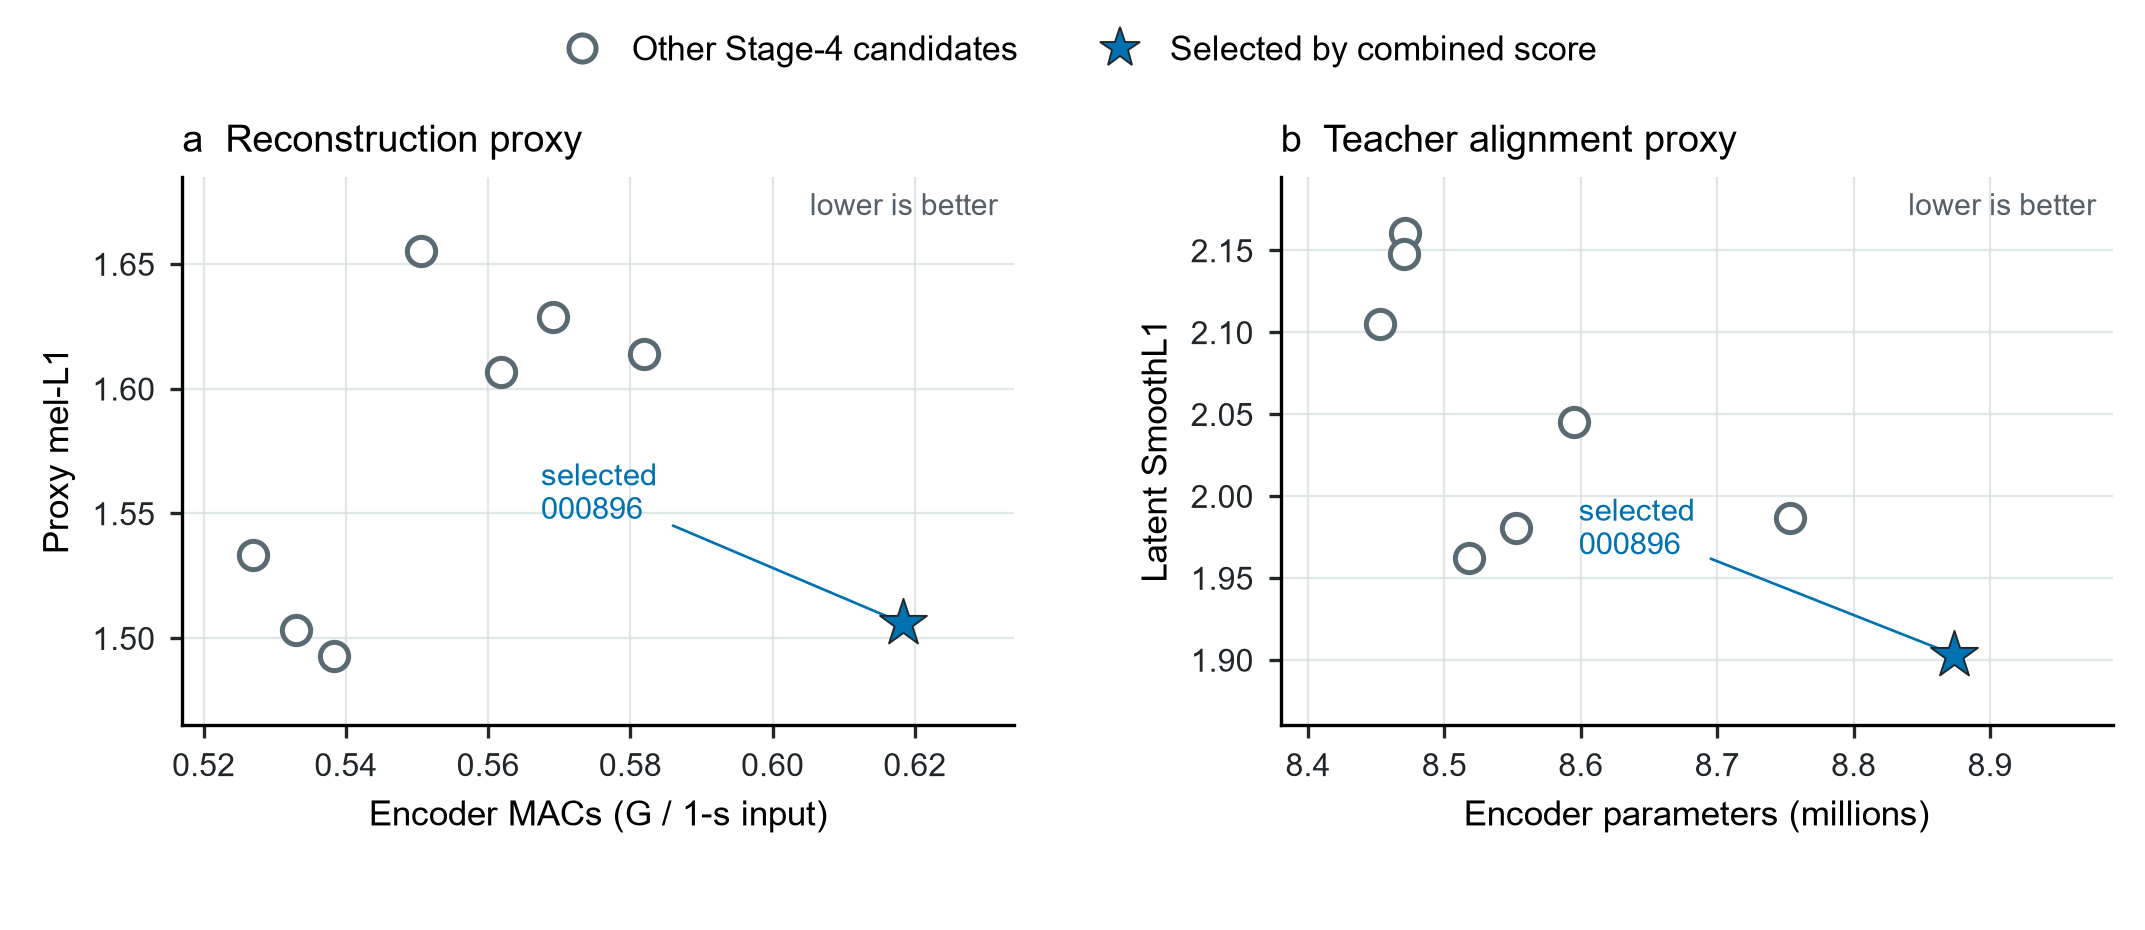
\includegraphics[width=\textwidth]{supplementary_methods_v3_assets/nas_finalists.png}
\caption{Quality--resource views of the eight final-stage NAS candidates. \textbf{a}, Encoder MACs against proxy mel-L1 measured with the frozen teacher downstream modules. \textbf{b}, Encoder parameters against latent SmoothL1 teacher-alignment loss. The star marks the architecture selected by the combined multimetric quality--resource score. These 32-utterance, 1,500-step search-stage proxies are not final SCIT reconstruction measurements; the resource measurements here describe these final-stage candidates and are not substituted for the initial-profile values reported in Results.}
\label{fig:sv4-nas-finalists}
\end{figure*}
% END V4-NAS-FIGURE

\subsection{Profiling and reduction calculations}
Encoder profiling used an NVIDIA GeForce RTX 5070 Ti, FP32, PyTorch 2.9.1 with CUDA 12.8, and THOP 0.1.1. The input was a batch of one Gaussian waveform with shape $1\times1\times16000$. Parameter counts were calculated from the encoder parameters, and THOP estimated multiply--accumulate operations for that input.

After the profiling forward pass and one explicit warm-up, five inference passes were timed with CUDA synchronization. For elapsed times $\tau_1,\ldots,\tau_5$ and input duration $d=1$~s,
\begin{equation}
 \mathrm{RTF}=\frac{1}{5d}\sum_{r=1}^{5}\tau_r.
 \label{eq:sv2-rtf}
\end{equation}
The measured operation was the encoder forward pass. Quantization, waveform decoding and speaker-classifier processing were separate components of the inference pipeline.

The Results resource comparison uses the initial profiling records for the reference and the selected candidate: 67,705,856 versus 8,873,360 parameters; 5,869,363,200 versus 618,393,600 MACs; and RTF 0.00818658 versus 0.00367646. For each quantity $q$, the relative reduction was
\begin{equation}
 \rho_q=100\left(1-\frac{q_{\rm selected}}{q_{\rm reference}}\right)\%.
 \label{eq:sv2-reduction}
\end{equation}
Rounding these ratios to one decimal place yields 86.9\%, 89.5\% and 55.1\%, respectively. The plot of 8,192 profiles and the normalized resource comparison in Results use these same records.

% BEGIN V3-ENCODER
\subsection{Layerwise structure of the selected encoder}
Table~\ref{tab:sv3-encoder} specifies the selected encoder in execution order. Here $N$ is a waveform length divisible by 320; a one-second input therefore reaches successive temporal lengths of 16,000, 3,200, 800, 200 and 50. The implementation applies reflection padding around noncausal convolutions, with additional right padding when needed to complete a stride. For other input lengths, the actual tensor length is retained by the processing and cache metadata.

\begin{table*}[t]
\centering
\caption{Selected waveform encoder, in execution order. Shapes use batch size $B$ and input length $N$ divisible by 320. Each downsampling convolution follows a Snake activation.}
\label{tab:sv3-encoder}
\small
\begin{tabularx}{\textwidth}{@{}p{0.16\textwidth}Yp{0.18\textwidth}p{0.19\textwidth}@{}}
\toprule
Module & Operation & Channels & Output shape\\
\midrule
Input convolution & Kernel 7, stride 1 & $1\rightarrow24$ & $B\times24\times N$\\
Residual position 1 & Identity & $24\rightarrow24$ & $B\times24\times N$\\
Downsampling 1 & Kernel 10, stride 5 & $24\rightarrow48$ & $B\times48\times(N/5)$\\
Residual position 2 & Standard convolution, kernel 7 & $48\rightarrow48$ & $B\times48\times(N/5)$\\
Downsampling 2 & Kernel 8, stride 4 & $48\rightarrow96$ & $B\times96\times(N/20)$\\
Residual position 3 & Depthwise kernel 9, then pointwise kernel 1 & $96\rightarrow96$ & $B\times96\times(N/20)$\\
Downsampling 3 & Kernel 8, stride 4 & $96\rightarrow192$ & $B\times192\times(N/80)$\\
Residual position 4 & Kernel 5, dilation 2 & $192\rightarrow192$ & $B\times192\times(N/80)$\\
Downsampling 4 & Kernel 8, stride 4 & $192\rightarrow384$ & $B\times384\times(N/320)$\\
Recurrent block & One bidirectional LSTM; 384 hidden units per direction & $384\rightarrow768$ & $B\times768\times(N/320)$\\
Output projection & Snake, then kernel-7 convolution & $768\rightarrow1024$ & $B\times1024\times(N/320)$\\
\bottomrule
\end{tabularx}
\end{table*}

Convolutions use weight normalization. Each non-identity residual operator is followed by one-group normalization and Snake activation before addition to its input; none uses squeeze-and-excitation. The separable operator preserves the channel count during its depthwise and pointwise steps. The bidirectional recurrent block concatenates its two directional outputs and adds the input duplicated along the feature axis. The final projection therefore receives 768, rather than 384, channels. These settings describe the architecture subsequently used in both SCIT and SCIT-LCA.
% END V3-ENCODER

\section{Codec training}
\label{sec:sv2-training}

\subsection{Data preparation and model initialization}
The base codec used 27,039 training utterances and 1,500 disjoint validation utterances from LibriSpeech train-clean-100~\cite{librispeech}. Membership was fixed by the retained file manifests. Training examples were random one-second waveform crops with the corresponding intervals of precomputed teacher features. Inputs shorter than the target crop were zero-padded. Validation used deterministic first-30-second segments, padding shorter utterances, at batch size one.

The selected NAS encoder, the three RVQ codebooks and the decoder were trained jointly from scratch. The decoder retained 64 initial filters, upsampling ratios $(8,5,4,2)$, two unidirectional LSTM layers and ELU activation. The 1024-dimensional quantizer interface connected the selected encoder to this decoder. Test-clean utterances belonged to the evaluation populations described in Section~\ref{sec:sv2-evaluation}.

Two teacher representations have distinct roles in this workflow. NAS aligns the candidate encoder to the pretrained SpeechTokenizer teacher's 1024-dimensional pre-quantization latents. Base codec training instead uses 768-dimensional HuBERT features to supervise the first quantizer. The latter supervision is provided by a learned 1024-to-768 projection.

\subsection{Waveform and multi-scale spectral objectives}
For reference and reconstructed signals truncated to their common sample length $N'$, waveform reconstruction loss was
\begin{equation}
 \mathcal L_{\rm wav}(x,\hat x)
 =\frac{1}{N'}\sum_{n=1}^{N'}|x_n-\hat x_n|,
 \label{eq:sv2-wav}
\end{equation}
with a further mean over the minibatch. Spectral reconstruction used four log-power mel representations. Let $\mathcal M_s(x)$ denote the log mel spectrogram at scale $s$. The multi-scale term was
\begin{equation}
 \mathcal L_{\rm mel}^{\rm ms}(x,\hat x)
 =\sum_{s=1}^{4}\alpha_s
     \operatorname{mean}|\mathcal M_s(x)-\mathcal M_s(\hat x)|.
 \label{eq:sv2-msmel}
\end{equation}
The FFT and window lengths were 1024, 512, 256 and 128 samples; hops were 240, 120, 60 and 30 samples; and $\alpha_s$ values were 45, 1, 1 and 1. All scales used 80 mel bands over 0--8~kHz, Hann windows, HTK mel spacing, Slaney filter normalization and an uncentred STFT. Mel power was floored at $10^{-9}$ before the natural logarithm. Spectrograms were truncated to their common frame length before calculating each mean absolute difference.

\begin{table}[t]
\centering
\caption{Spectral resolutions used in codec training. Evaluation mel-L1 uses the first row with unit weight.}
\label{tab:sv2-mels}
\small
\begin{tabular}{@{}rrrr@{}}
\toprule
FFT & Window & Hop & Training weight\\
\midrule
1024 & 1024 & 240 & 45\\
512 & 512 & 120 & 1\\
256 & 256 & 60 & 1\\
128 & 128 & 30 & 1\\
\bottomrule
\end{tabular}
\end{table}

\subsection{Adversarial learning and feature matching}
Multi-period, multi-scale waveform and multi-scale STFT discriminators supplied complementary waveform and spectral learning signals. Index discriminator outputs by $j$ and their intermediate feature maps by $F_{j,\ell}$. The discriminator loss was
\begin{equation}
 \mathcal L_D=\sum_j\left[
  \operatorname{mean}(1-D_j(x))^2
  +\operatorname{mean}D_j(\operatorname{sg}(\hat x))^2
 \right],
 \label{eq:sv2-disc}
\end{equation}
where $\operatorname{sg}$ denotes stop-gradient. Real speech had target one, and detached reconstructed speech had target zero. For the generator, the adversarial term was
\begin{equation}
 \mathcal L_{\rm adv}
 =\sum_j\operatorname{mean}(1-D_j(\hat x))^2.
 \label{eq:sv2-adv}
\end{equation}
Discriminator feature matching was
\begin{equation}
 \mathcal L_{\rm fm}
 =2\sum_{j,\ell}\operatorname{mean}
   |F_{j,\ell}(x)-F_{j,\ell}(\hat x)|.
 \label{eq:sv2-fm}
\end{equation}
The factor of two is part of the implemented feature-matching function. Generator and discriminator losses used separate optimizers.

\subsection{RVQ gradients and codebook updates}
Nearest-neighbour index selection is discrete. During the training forward pass, each quantized output was represented by a straight-through value
\begin{equation}
 q^{\rm ST}_{m,t}
 =r_{m-1,t}+\operatorname{sg}(q_{m,t}-r_{m-1,t}).
 \label{eq:sv2-ste}
\end{equation}
Its forward value is the selected codeword, and its backward derivative with respect to the layer input is the identity. The commitment term averaged squared differences between the layer input and the detached quantized value:
\begin{equation}
 \mathcal L_{\rm commit}
 =\frac{1}{3}\sum_{m=1}^{3}
   \operatorname{MSE}(r_{m-1},\operatorname{sg}(q_m)),
 \label{eq:sv2-commit}
\end{equation}
where the elementwise mean includes feature, frame and batch dimensions.

Each codebook was initialized by 50 iterations of $k$-means on its first training-batch inputs. Codebook embeddings were maintained as buffers and updated by exponential moving averages (EMA), with decay $\gamma=0.99$. For codeword $k$, let $n_k$ and $s_k$ be the current batch's assignment count and assigned-vector sum. The running statistics obeyed
\begin{align}
 N_k&\leftarrow\gamma N_k+(1-\gamma)n_k,\nonumber\\
 A_k&\leftarrow\gamma A_k+(1-\gamma)s_k.
 \label{eq:sv2-ema}
\end{align}
The codeword was obtained by dividing $A_k$ by its smoothed assignment count. With $\epsilon=10^{-5}$ and $N_{\rm all}=\sum_jN_j$, the normalized count was
\begin{equation}
 \widetilde N_k=
 \frac{N_k+\epsilon}{N_{\rm all}+K\epsilon}N_{\rm all}.
 \label{eq:sv2-ema-count}
\end{equation}
The implementation also checked for entries with EMA counts below two and replaced their embedding values with sampled vectors from the current batch before the EMA update. Encoder and decoder parameters followed gradient-based optimization, while these assignment statistics controlled codebook updates.

\subsection{HuBERT supervision and combined loss}
Semantic features were precomputed with the fixed \textit{facebook/hubert-base-ls960} model~\cite{hubert}, averaging its returned hidden states. Let $h_t\in\mathbb{R}^{768}$ denote the teacher feature and $P:\mathbb{R}^{1024}\rightarrow\mathbb{R}^{768}$ the learned projection of the first RVQ output. After truncation to the common feature length $T'$, the semantic objective was
\begin{equation}
 \mathcal L_{\rm sem}
 =-\frac{1}{T'}\sum_{t=1}^{T'}
       \log\sigma\!\left(\cos(Pq_{1,t},h_t)\right),
 \label{eq:sv2-sem}
\end{equation}
with a mean over the minibatch and $\sigma$ the logistic sigmoid. This term provides a feature-alignment signal alongside the waveform-domain objectives.

The full generator objective was
\begin{equation}
\begin{split}
 \mathcal L_{\rm base}={}&
 500\mathcal L_{\rm wav}
 +\mathcal L_{\rm mel}^{\rm ms}
 +\mathcal L_{\rm adv}+\mathcal L_{\rm fm}\\
 &+10\mathcal L_{\rm commit}+30\mathcal L_{\rm sem}.
\end{split}
\label{eq:sv2-base}
\end{equation}
The multi-scale mel weights in Table~\ref{tab:sv2-mels} are already included in $\mathcal L_{\rm mel}^{\rm ms}$. The commitment weight is applied after averaging the three layer losses.

\subsection{Optimization and checkpoint selection}
The recorded base run used seed 42, minibatches of eight, bfloat16 mixed precision and separate Adam optimizers for the generator and discriminators. Both optimizers used initial learning rate $10^{-4}$, $\beta=(0.9,0.99)$ and zero weight decay. Cosine schedules used zero warm-up and a configured 60-epoch horizon.

Training reached 122,500 minibatch steps. The minimum validation mel loss selected the checkpoint at step 107,500, which was retained as SCIT. This selected checkpoint initialized the channel-adaptation stage and supplied the SCIT row in the matched-rate reconstruction comparison. Recording the selected step alongside the run endpoint identifies the precise model used in each subsequent experiment.

% BEGIN V3-TRAINING
\subsection{Training-stage summary and model handoff}
Table~\ref{tab:sv3-training-stages} places the four learning stages in a common format. Architecture selection transfers the configuration to base training. Base training transfers generator weights to channel adaptation. The retained adapted checkpoint then generates the fixed token--waveform cache used by the speaker classifiers. Thus, each transition has an explicit transferred object, while each stage keeps its own optimization and selection rule.

\begin{table*}[t]
\centering
\caption{Training stages and retained model states. Steps in the codec rows are recorded minibatch steps. The classifier uses the explicit eight-minibatch accumulation rule in Section~\ref{sec:sv2-speaker-protocol}.}
\label{tab:sv3-training-stages}
\small
\begin{tabularx}{\textwidth}{@{}>{\raggedright\arraybackslash}p{0.12\textwidth}>{\raggedright\arraybackslash}p{0.20\textwidth}Y>{\raggedright\arraybackslash}p{0.23\textwidth}@{}}
\toprule
Stage & Input and initialization & Optimization and updated components & Selection and transferred object\\
\midrule
NAS alignment & One-second crops, batch 1; fresh candidate initialization per stage & AdamW, $10^{-4}$; 100/500/1,500 steps; candidate encoder trained against a frozen teacher & Combined final ranking score; selected architecture configuration\\
Base SCIT & One-second crops, batch 8; encoder, codebooks and decoder initialized for joint training & Adam, $10^{-4}$, bfloat16; configured 60-epoch schedule; 122,500 recorded steps; generator/discriminator gradients and codebook EMA & Lowest validation mel loss; generator checkpoint at step 107,500\\
SCIT-LCA & Same codec data, batch 8; SCIT generator weights; new discriminator and optimizer states & Adam, $10^{-5}$, bfloat16; ten epochs, 32,500 steps; full-depth and sampled communication objectives & Validation communication mel loss; generator checkpoint at step 30,000\\
Speaker classifier & Frozen SCIT-LCA cache; crops up to three seconds; batch 16; seeds 41/42/43 & AdamW, 30 epochs; $3\times10^{-4}$ for token/fusion modules and $10^{-4}$ for projection/heads; codec and ECAPA frozen & Highest validation macro-F1; then validation-only temperature fitting\\
\bottomrule
\end{tabularx}
\end{table*}

Codebook updates in the two codec stages use the EMA assignment statistics in Section~\ref{sec:sv2-training}, rather than an optimizer applied to codeword parameters. The first-layer semantic projection is trained with the generator while the HuBERT targets remain fixed. In the downstream stage, cached speech representations are read without reopening codec optimization. The three speaker runs share the data split and upstream checkpoint, and differ in classifier training seed.
% END V3-TRAINING

\section{Channel-aware fine-tuning}
\label{sec:sv2-lca}

\subsection{Initialization and sampled training conditions}
SCIT-LCA started from the selected SCIT generator weights. Its discriminator and optimizer states were initialized for the fine-tuning run. The architecture, codebook sizes, waveform sampling rate and latent interface were retained. Fine-tuning used the same codec training and validation manifests as the base stage.

Each training minibatch used a full-depth branch and an additional communication branch. The communication branch independently sampled $L$ uniformly from $\{1,2,3\}$ and one of five equally probable channel conditions: clean, 5\% erasure, 10\% erasure, 1\% substitution or 3\% substitution. The selected depth and condition applied to the minibatch; index-level masks were then sampled over the retained code tensor.

\begin{table}[t]
\centering
\caption{Training distribution for the communication branch. Each row has probability 0.2 and is combined with uniform depth sampling.}
\label{tab:sv2-lca-conditions}
\small
\begin{tabularx}{\columnwidth}{@{}lrrY@{}}
\toprule
Condition & $p_{\rm erase}$ & $p_{\rm sub}$ & Replacement\\
\midrule
Clean & 0 & 0 & Original indices\\
Erasure, medium & 0.05 & 0 & Previous original index\\
Erasure, high & 0.10 & 0 & Previous original index\\
Substitution, medium & 0 & 0.01 & Uniform legal index\\
Substitution, high & 0 & 0.03 & Uniform legal index\\
\bottomrule
\end{tabularx}
\end{table}

\subsection{Index perturbation operators}
For erasure, let $e_{m,t}$ be a Bernoulli mask with probability $p_{\rm erase}$, and set $e_{m,0}=0$. The replacement operator was
\begin{equation}
 \widetilde i_{m,t}=
 \begin{cases}
 i_{m,t-1}, & e_{m,t}=1,\ t>0,\\
 i_{m,t}, & \text{otherwise}.
 \end{cases}
 \label{eq:sv2-erasure}
\end{equation}
The predecessor is taken from the original index sequence. For example, applying a mask to the last two entries of $(a,b,c,d)$ yields $(a,b,b,c)$. This example specifies the simultaneous one-frame-shift replacement used by the implementation. The first frame remains unchanged.

For substitution, let $s_{m,t}\sim\operatorname{Bernoulli}(p_{\rm sub})$ and draw $u_{m,t}$ uniformly from $\{0,\ldots,1023\}$. Then
\begin{equation}
 \widetilde i_{m,t}=
 \begin{cases}
 u_{m,t}, & s_{m,t}=1,\\
 i_{m,t}, & s_{m,t}=0.
 \end{cases}
 \label{eq:sv2-substitution}
\end{equation}
A legal replacement can equal the original index. Thus, $p_{\rm sub}$ specifies the selection probability for substitution, rather than enforcing a different value at every selected position. The training conditions apply erasure or substitution separately.

\subsection{Communication and consistency objectives}
Let $\hat x_L^{\,c}$ and $\hat x_L^{\,p}$ denote clean and perturbed decodes at the same sampled depth. The communication branch minimized reconstruction error against the reference waveform and, for a perturbed condition, disagreement with the clean decode:
\begin{equation}
\begin{split}
 \mathcal L_{\rm comm}={}&
 500\mathcal L_{\rm wav}(x,\hat x_L^{\,p})
 +\mathcal L_{\rm mel}^{\rm ms}(x,\hat x_L^{\,p})\\
 &+0.5\mathcal L_{\rm cons},
\end{split}
\label{eq:sv2-comm}
\end{equation}
where
\begin{equation}
 \mathcal L_{\rm cons}=
 \begin{cases}
 \mathcal L_{\rm mel}^{\rm ms}(\hat x_L^{\,c},\hat x_L^{\,p}),
       & \text{perturbed condition},\\
 0,    & \text{clean condition}.
 \end{cases}
 \label{eq:sv2-consistency}
\end{equation}
All spectral terms use the resolutions and weights in Table~\ref{tab:sv2-mels}. The full objective was
\begin{equation}
 \mathcal L_{\rm LCA}
 =\mathcal L_{\rm base}+1.5\mathcal L_{\rm comm}.
 \label{eq:sv2-lca}
\end{equation}
The full-depth branch preserves the base reconstruction, adversarial, commitment and semantic objectives. The communication branch supplies additional reconstruction training on the sampled received-index condition.

\subsection{Gradient routing and update sequence}
For each minibatch, the full-depth forward pass generated the reconstruction and semantic features used by $\mathcal L_{\rm base}$. Discriminator updates used the real waveform and the detached full-depth reconstruction. The generator update then combined the full-depth and communication objectives.

The code tensor for the communication branch was obtained by a separate encoder-and-index extraction call without gradient tracking. It was truncated to the sampled depth and perturbed before codebook lookup and waveform decoding. Consequently, the communication losses backpropagated through the decoder; the full-depth branch supplied encoder gradients and quantizer training updates. The clean decode in the consistency term was not detached, so both decodes contributed gradients to their shared decoder.

This update sequence retains the reconstruction and semantic learning signals while exposing the decoder to alternative index inputs. Packet and burst masks were introduced in the evaluation protocol in Section~\ref{sec:sv2-evaluation}; the fine-tuning distribution was the five-condition distribution in Table~\ref{tab:sv2-lca-conditions}.

\subsection{Fine-tuning configuration and retained model}
Fine-tuning used seed 42, minibatches of eight, bfloat16 precision, initial learning rate $10^{-5}$ and zero warm-up. The recorded run comprised 32,500 minibatch steps over its ten-epoch schedule. The step-30,000 checkpoint was selected using validation communication-branch mel loss, including the 3\% substitution condition at all three sampled depths.

This checkpoint is the SCIT-LCA model used in the reported clean and perturbed reconstruction comparisons and in the speaker-cache generation. The evaluation depth was fixed at $L=3$ for all of those measurements. The checkpoint identity connects channel adaptation directly to the frozen representation used by the downstream task.

% BEGIN V3-ALGORITHM
\subsection{Minibatch computation and update procedure}
Algorithm~\ref{alg:sv3-lca} connects the objectives above to their execution order. The full-depth forward pass supplies differentiable encoder features and the RVQ training updates. The separate index-extraction call supplies integer inputs for the communication path. Only the selected depth and channel condition are shared across a minibatch; perturbation masks are sampled over index positions.

\begin{algorithm}[t]
\caption{One SCIT-LCA minibatch}
\label{alg:sv3-lca}
\small
\begin{tabularx}{\columnwidth}{@{}rY@{}}
\toprule
 & \textbf{Input:} waveform batch $x$, aligned HuBERT targets, current generator and discriminators.\\
\midrule
1 & Run the full three-layer generator forward pass; retain reconstructed speech, semantic features and commitment loss.\\
2 & Clear discriminator gradients. Evaluate $\mathcal L_D$ on $x$ and the detached full-depth reconstruction.\\
3 & Backpropagate $\mathcal L_D$; update the discriminator optimizer and scheduler when gradient synchronization is active.\\
4 & Evaluate the full-depth generator objective $\mathcal L_{\rm base}$ with the current discriminator outputs.\\
5 & Sample $L\in\{1,2,3\}$ uniformly and one channel condition from Table~\ref{tab:sv2-lca-conditions}.\\
6 & Without gradient tracking, encode $x$ into integer indices and retain the first $L$ rows, denoted $I_L$.\\
7 & Apply the selected perturbation to obtain $\widetilde I_L$; decode it to $\hat x_L^{\,p}$.\\
8 & If perturbed, also decode $I_L$ to $\hat x_L^{\,c}$ and evaluate $\mathcal L_{\rm cons}$ without detaching either decode. Otherwise set $\mathcal L_{\rm cons}=0$.\\
9 & Form $\mathcal L_{\rm comm}$ using Equation~\ref{eq:sv2-comm}, then $\mathcal L_{\rm base}+1.5\mathcal L_{\rm comm}$.\\
10 & Backpropagate the combined generator loss. When gradient synchronization is active, update its optimizer and scheduler and clear generator gradients.\\
\bottomrule
\end{tabularx}
\end{algorithm}

The synchronization condition in the algorithm follows the training loop's optimizer-step gate; a minibatch count is recorded separately from an optimizer update. Both communication decodes use the same decoder parameters and the same retained clean indices. The consistency term consequently compares two received-index conditions at a common depth. HuBERT feature extraction is performed before training and is not an additional forward branch in this iteration.
% END V3-ALGORITHM

\section{Reconstruction and token-domain robustness evaluation}
\label{sec:sv2-evaluation}

\subsection{Evaluation populations and waveform processing}
The external-codec comparison used the first 300 entries of the retained LibriSpeech test-clean manifest, in its recorded order. The paired comparison between SCIT and SCIT-LCA used all 2,620 test-clean utterances. Each experiment retained utterance identifiers, codec settings and metric values so that aggregation could be reproduced for its own evaluation population.

\begin{table}[t]
\centering
\caption{Evaluation populations supporting the main results.}
\label{tab:sv2-populations}
\small
\begin{tabularx}{\columnwidth}{@{}lY@{}}
\toprule
Experiment & Population and unit\\
\midrule
External-codec comparison & First 300 test-clean utterances; equal utterance weights\\
SCIT/SCIT-LCA comparison & All 2,620 test-clean utterances; matched utterance and perturbation\\
Speaker identification & 1,650 VCTK test utterances; 15 per identity; three training seeds\\
\bottomrule
\end{tabularx}
\end{table}

Reconstruction models ran in evaluation mode without gradient tracking and processed complete utterances. Reference and reconstructed waveforms were represented as mono 16-kHz signals. Each pair was truncated to its common sample length before metrics were calculated. Metric preprocessing used this common-length truncation without an additional delay-search or waveform-alignment optimization.

The 300-utterance and 2,620-utterance averages are calculated over their respective populations. For example, the SCIT clean reconstruction value in an external-codec table and that in a full-set adaptation table refer to different sets of utterances. The retained population identifier is therefore part of the definition of each reported mean.

\subsection{External codec settings}
The matched-rate learned baselines were the pretrained 16-kHz DAC model with three active quantizers~\cite{dac} and the pretrained 24-kHz EnCodec model at its 1.5-kbit/s setting~\cite{encodec}. EnCodec inputs were resampled from 16 to 24~kHz, and its reconstructions were resampled back to 16~kHz for scoring. DAC and SCIT were evaluated at 16~kHz.

The conventional-codec reference used FFmpeg/libopus at a requested bitrate of 6~kbit/s, with mono 16-kHz decoded output. PCM passthrough at 256~kbit/s supplied the uncompressed reference. The external codec checkpoints were used without fine-tuning on the comparison population. The archived setting labels identify SCIT as \texttt{L=3}, DAC as \texttt{n\_q\_3}, EnCodec as \texttt{bw1.5kbps\_n\_cb2}, Opus as \texttt{opus\_6000bps} and PCM as \texttt{16bit\_16khz\_passthrough}.

Nominal rates identify these operating points. Finite-utterance padding, byte alignment and container fields belong to the corresponding stored payload records. For low-rate Opus, full-band mel-L1 is sensitive to bandwidth reduction; spectral error is therefore read together with the intelligibility and perceptual-quality metrics.

\subsection{Metric definitions and aggregation}
Evaluation mel-L1 used the 1024-sample FFT and window, 240-sample hop and 80-band, 0--8-kHz log-power mel representation. HTK mel spacing, Slaney normalization, a $10^{-9}$ floor and an uncentred STFT matched the corresponding spectral preprocessing in training. Its score was the unweighted mean absolute spectrogram difference:
\begin{equation}
 d_{\rm mel}(x,\hat x)
 =\operatorname{mean}|\mathcal M_1(x)-\mathcal M_1(\hat x)|.
 \label{eq:sv2-evalmel}
\end{equation}
This is a single-scale evaluation score; the factor 45 and the three additional resolutions belong to the training objective in Equation~\ref{eq:sv2-msmel}.

Short-time objective intelligibility (STOI) used the non-extended implementation~\cite{stoi}. PESQ used wideband mode at 16~kHz~\cite{pesq}. Lower mel-L1 and higher STOI and PESQ-WB indicate better values under their respective metric definitions. Metrics were calculated per utterance. For values $d_1,\ldots,d_n$, the reported mean was
\begin{equation}
 \bar d=\frac{1}{n}\sum_{u=1}^{n}d_u.
 \label{eq:sv2-mean}
\end{equation}
Thus, each utterance had equal weight, independently of duration.

For the 300-utterance comparison, each metric's 95\% interval was computed by drawing 10,000 nonparametric bootstrap samples with seed 42. Each draw sampled 300 utterance indices with replacement and recomputed the mean. The 2.5th and 97.5th percentiles of the bootstrap means supplied the lower and upper endpoints. These intervals describe resampling variability within the specified comparison population.

\subsection{Independent and temporally grouped masks}
The full-set evaluation included clean transmission, independent 10\% erasure, independent 3\% substitution, five-frame packet masks at probability 0.05, and one ten-frame burst per utterance. All conditions used $L=3$. Independent masks operated over individual layer--frame positions. Their replacements followed Equations~\ref{eq:sv2-erasure} and~\ref{eq:sv2-substitution}.

For packet masks, frames were partitioned into non-overlapping groups of five, starting at the first frame; a final short group was retained. Each group was selected with probability 0.05. The resulting temporal mask was broadcast across all three RVQ layers. At a 50-Hz frame rate, five frames correspond to 100~ms. The first frame was protected by the replacement operator.

For the burst condition, the mask covered one contiguous span of ten frames, corresponding to 200~ms. For an utterance with $T_q>10$ frames, the start was sampled uniformly from zero-based positions 1 through $T_q-10$, inclusive. For a shorter sequence, the span length was reduced to the sequence length and frame zero was protected. The same span was applied across all layers.

Both grouped conditions used the preceding original index at masked positions, following Equation~\ref{eq:sv2-erasure}. The five-frame and ten-frame definitions specify temporal correlation in the mask, while the replacement operator specifies the code values actually decoded. These definitions are the token-domain perturbations underlying the packet and burst rows in Results.

\subsection{Pairing and adaptation differences}
SCIT and SCIT-LCA were evaluated on matched utterances with the same sampled masks for each depth and condition. The base seed was 42 for independent index perturbations and 123 for packet and burst perturbations. The metric records retain the resolved channel seed for each utterance--depth--condition pair; replay uses that recorded seed with the same generator device and index shape.

For metric $d$, the utterance-level adaptation difference was
\begin{equation}
 \Delta d_u=d_u^{\rm LCA}-d_u^{\rm SCIT},
 \qquad
 \overline{\Delta d}=\frac{1}{2620}\sum_{u=1}^{2620}\Delta d_u.
 \label{eq:sv2-paired}
\end{equation}
Negative mel-L1 differences and positive STOI or PESQ-WB differences favour SCIT-LCA. The shared condition and seed pair the perturbation realization while the independently trained codec checkpoints supply their own indices and reconstructions. All reported test-condition comparisons use the retained checkpoints selected on validation data.

% BEGIN V3-PERTURBATION
\subsection{Worked index examples and temporal support}
Figure~\ref{fig:sv3-perturbations} separates the mask pattern from the rule that supplies replacement values. For the illustrative row $(13,44,72,31,86,9)$, masking zero-based positions 2 and 3 gives $(13,44,44,72,86,9)$: both replacements read the original row. A random substitution instead supplies an independently sampled legal codeword index at each selected position. These numerical examples illustrate the operations and are not sampled experimental outcomes.

\begin{figure*}[t]
\centering
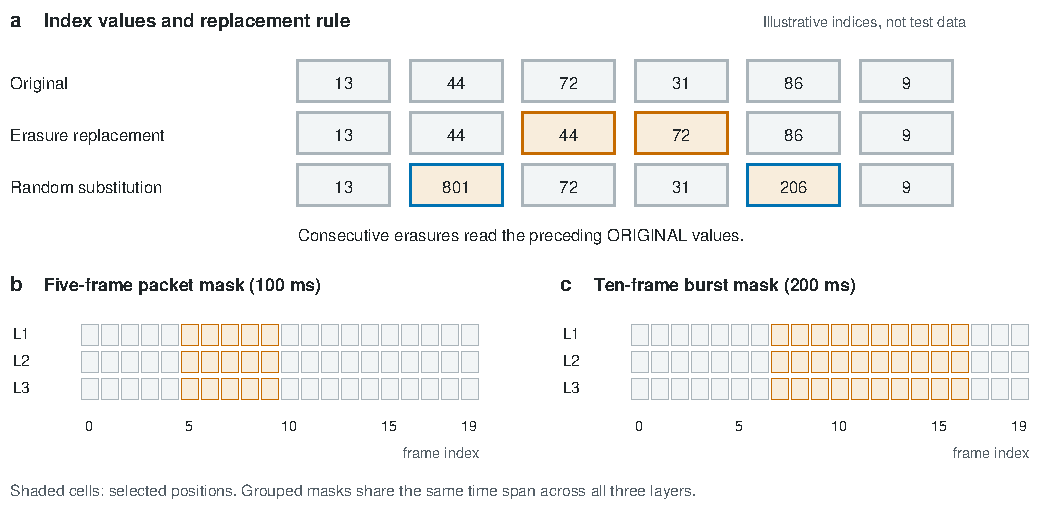
\includegraphics[width=\textwidth]{supplementary_methods_v3_assets/index_perturbations.pdf}
\caption{Index replacement and temporally grouped masks. \textbf{a}, Consecutive erased positions use their preceding original indices, whereas substitution draws legal index values. Highlighted cells identify selected positions. \textbf{b}, An illustrative selected five-frame group spans 100~ms. \textbf{c}, An illustrative ten-frame burst spans 200~ms. The grouped masks in b and c cover the same temporal positions in all three RVQ layers. Frame zero is protected by the erasure-replacement operator. The diagrams specify the evaluation protocol; they do not depict measured packet traces.}
\label{fig:sv3-perturbations}
\end{figure*}

Independent masks can select different positions in different layers. Grouped masks instead select temporal intervals and broadcast them across the three layers. A selected five-frame group therefore covers 15 layer--frame positions, and a ten-frame span covers 30, before applying first-frame protection. The time lengths follow the nominal 20-ms latent grid; selection probability, span length and replacement value remain separately specified parts of the protocol.
% END V3-PERTURBATION

% BEGIN V4-ROBUSTNESS-TEXT
Figure~\ref{fig:sv4-paired-robustness} shows the paired SCIT-LCA minus SCIT differences defined above at the evaluated $L=3$ setting. The mean PESQ-WB difference is negative under clean transmission and the two temporally grouped masks, whereas the independent erasure and substitution conditions have positive means. The display is descriptive and does not turn the paired differences into a claim of uniform benefit or statistical significance.
% END V4-ROBUSTNESS-TEXT

% BEGIN V4-ROBUSTNESS-FIGURE
\begin{figure*}[t]
\centering
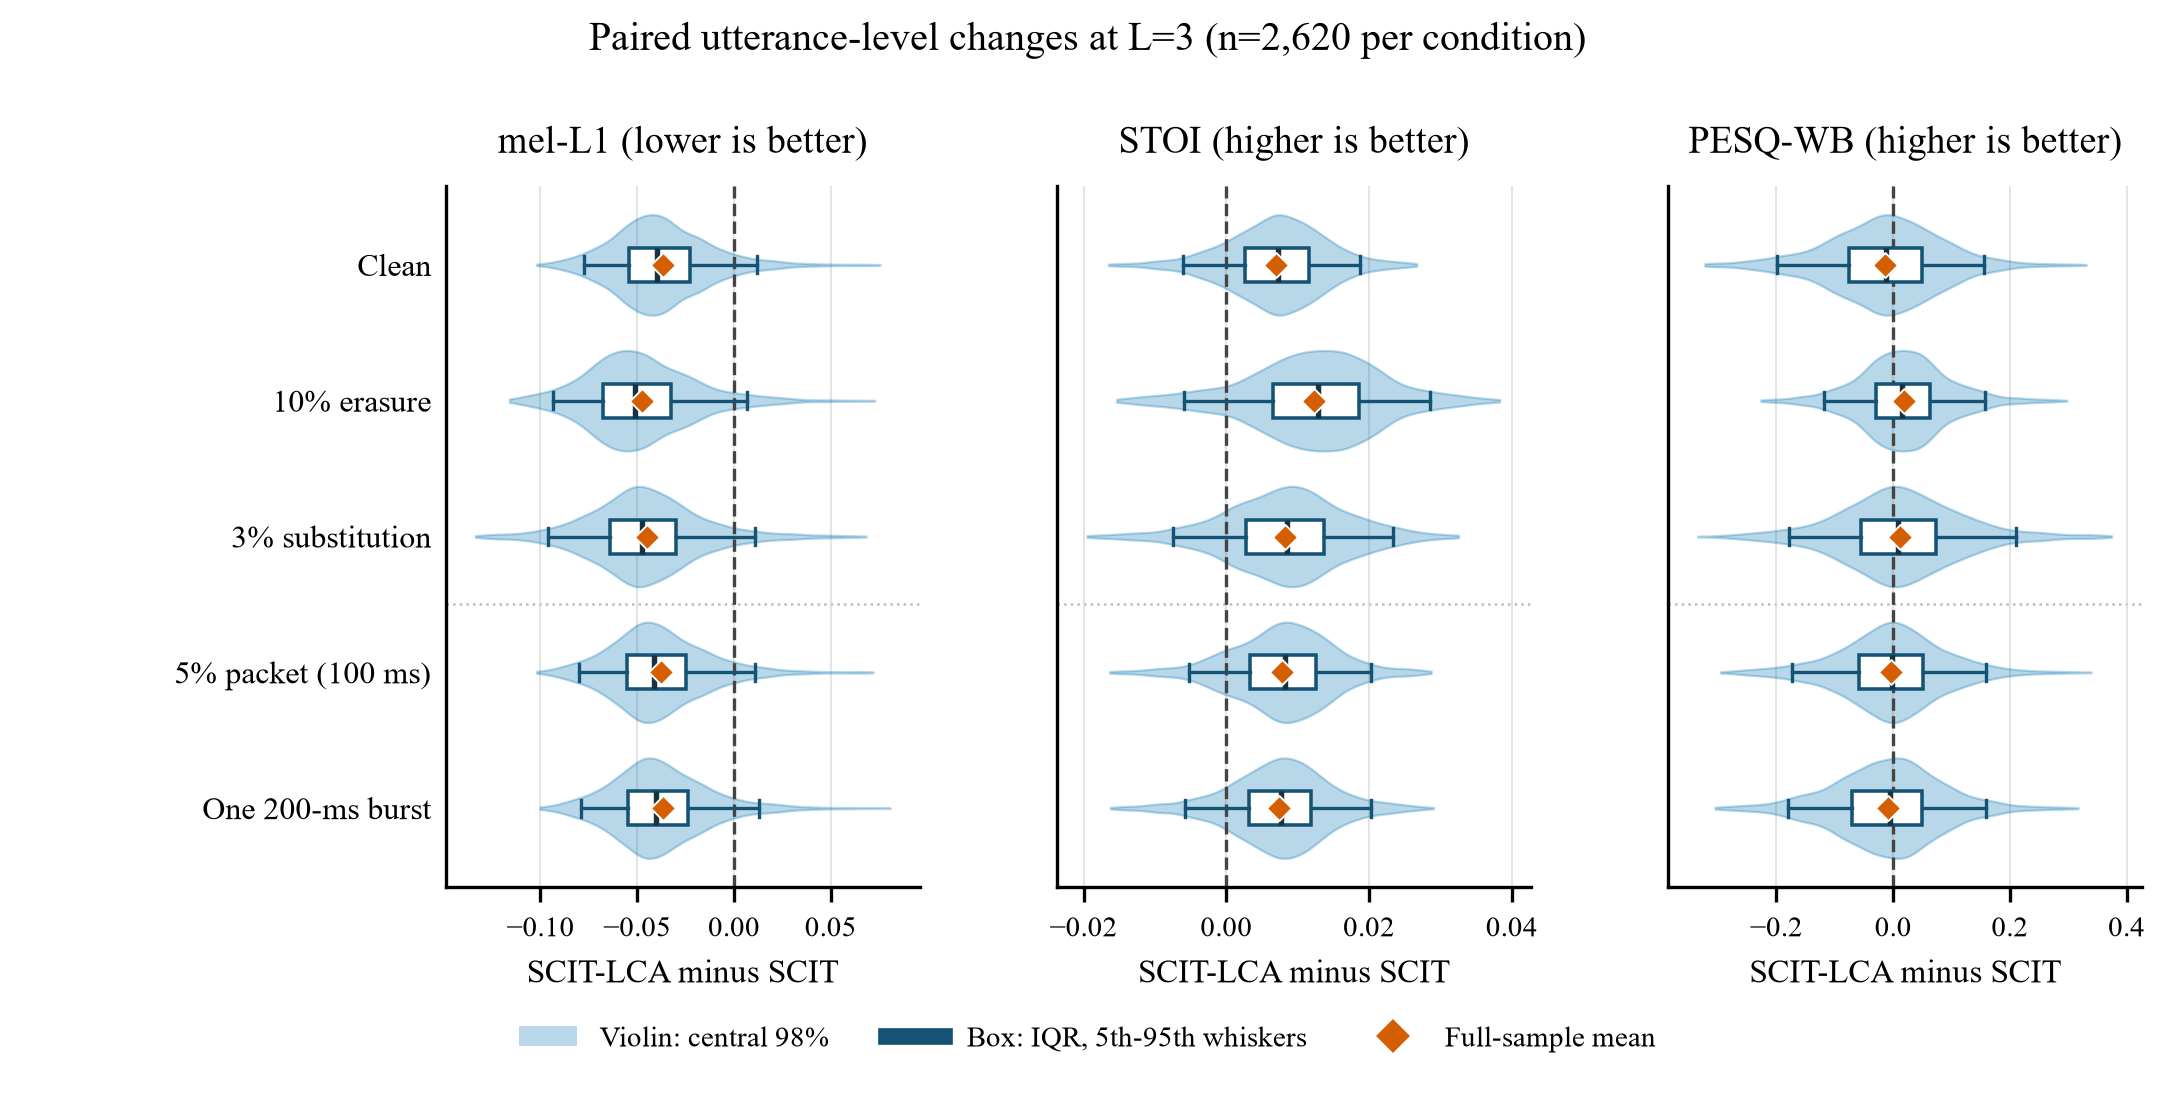
\includegraphics[width=\textwidth]{supplementary_methods_v3_assets/paired_robustness.png}
\caption{Utterance-level SCIT-LCA minus SCIT differences on the same 2,620 LibriSpeech test-clean utterances per condition at $L=3$. The five conditions comprise clean transmission, 10\% independent erasure, 3\% independent substitution, 5\% five-frame packet masking and one 200-ms burst. Each model pair is matched by utterance and channel seed. Diamonds show means over all 2,620 differences; boxes show interquartile ranges with 5th--95th-percentile whiskers, while violin densities display only the central 98\% to limit the influence of extreme tails on the plotting range. The dashed line indicates zero; lower mel-L1 and higher STOI/PESQ-WB are favourable. No significance test is implied.}
\label{fig:sv4-paired-robustness}
\end{figure*}
% END V4-ROBUSTNESS-FIGURE

\section{Frozen-codec speaker classifier}
\label{sec:sv2-speaker}

\subsection{Frozen inputs and cache construction}
The speaker experiment used the selected SCIT-LCA checkpoint at $L=3$. Before classifier training, each complete source utterance was resampled to mono 16~kHz, encoded into its three-layer indices and decoded into the corresponding waveform. The codec ran in evaluation and inference modes, and its parameters were excluded from downstream optimization.

The cache stored the index array, reconstructed waveform, source identity, utterance-group identifier, split membership, class index, valid waveform length, code-frame count and hashes of the codec checkpoint and configuration. State-dict hashes before and after cache construction were identical. This establishes the fixed codec state used to generate the classifier inputs. The recorded cache-failure list was empty.

The token and audio branches consume two representations of the same cached interval. Neither branch requires an independently transmitted speaker vector. Padding indices and masks are introduced by downstream batching and are not part of the ten-bit speech alphabet.

\subsection{Token embeddings and temporal processing}
Each RVQ layer has a separate embedding table with 1025 rows and 128 columns. Indices 0--1023 represent codewords; index 1024 is reserved for padding. A learned 128-dimensional layer embedding is added to each token embedding. For active-layer indicator $\ell_m$, table lookup $V_m[i_{m,t}]$ and layer embedding $e_m$, the combined feature is
\begin{equation}
 u_t=
 \frac{\sum_{m=1}^{3}\ell_m(V_m[i_{m,t}]+e_m)}
      {\max(1,\sum_{m=1}^{3}\ell_m)}.
 \label{eq:sv2-layer-mean}
\end{equation}
An affine projection maps $u_t$ to 256 channels. Frame masks zero padded positions after projection and after each temporal block.

The temporal encoder consists of four residual blocks with dilations 1, 2, 4 and 8. Each block uses a kernel-3, 256-channel depthwise convolution, GELU, a pointwise convolution and group normalization with one group. A residual addition and GELU are followed by the frame mask. With $\mathrm{DW}_d$ denoting depthwise convolution at dilation $d$, the block can be written
\begin{equation}
 h'=\mathrm{GELU}\!\left(
 h+\mathrm{GN}\!\left(
 \mathrm{PW}(\mathrm{GELU}(\mathrm{DW}_d(h)))
 \right)\right)\odot m_{\rm frame}.
 \label{eq:sv2-temporal}
\end{equation}
Padding equals the dilation, so the temporal length is preserved. The active-layer average permits the same temporal network to receive the layer masks sampled during training.

\subsection{Attentive statistics pooling}
For final temporal features $h_t\in\mathbb{R}^{256}$, a pointwise attention network maps 256 channels to 128, applies $\tanh$, and maps to one scalar score per frame. Padded-frame scores are set to $-10^4$ before the temporal softmax. The attention weights and pooled moments are
\begin{align}
 \alpha_t&=\frac{\exp(a_t)}{\sum_{\tau}\exp(a_\tau)},\nonumber\\
 \mu&=\sum_t\alpha_t h_t,\nonumber\\
 \sigma_h&=\sqrt{\max\left(
           \sum_t\alpha_t(h_t-\mu)^2,10^{-6}\right)}.
 \label{eq:sv2-pooling}
\end{align}
The maximum and square root are elementwise. Concatenating the 256-dimensional mean and standard deviation gives 512 features. A learned affine 512-to-256 projection and $\ell_2$ normalization yield the token embedding $z_{\rm tok}$.

Pooling combines information across the available speech interval while preserving a fixed embedding dimension. The attention mask uses the actual cached code length of the cropped item, enabling variable-duration utterances to share a batch.

\subsection{Audio embedding and gated fusion}
The audio branch uses the pretrained SpeechBrain \textit{spkrec-ecapa-voxceleb} ECAPA-TDNN model~\cite{ecapa}. Its preprocessing uses 80-bin filter-bank features and utterance-level mean normalization. The formal runs keep the ECAPA backbone frozen and in evaluation mode. A trainable affine projection maps its 192-dimensional embedding to 256 dimensions, followed by $\ell_2$ normalization to obtain $z_{\rm aud}$.

The two embeddings are combined by a vector-valued gate:
\begin{align}
 g&=\sigma\!\left(W_g[z_{\rm tok};z_{\rm aud}]+b_g\right),
 \nonumber\\
 v&=g\odot P_t(z_{\rm tok})+(1-g)\odot P_a(z_{\rm aud}),
 \nonumber\\
 z_{\rm fus}&=\operatorname{norm}_2(\operatorname{LN}(v)).
 \label{eq:sv2-gate}
\end{align}
Here $g\in(0,1)^{256}$, $P_t$ and $P_a$ are learned affine 256-to-256 projections, $\operatorname{LN}$ is layer normalization and $\odot$ denotes elementwise multiplication. The gate is calculated from the concatenated token and audio embeddings. Its dimensionality allows each fused feature to have its own mixing coefficient.

\begin{table}[t]
\centering
\caption{Classifier modules and parameter status during the formal speaker runs.}
\label{tab:sv2-speaker-modules}
\small
\begin{tabularx}{\columnwidth}{@{}YY@{}}
\toprule
Module & Configuration and status\\
\midrule
SCIT-LCA & Three-layer codec; frozen\\
Token embeddings & Three $1025\times128$ tables; trainable\\
Token temporal network & 256 channels; four dilated residual blocks; trainable\\
Token pooling & Attentive mean and standard deviation; 512-to-256 projection\\
ECAPA-TDNN & 192-dimensional output; frozen\\
Audio projection & 192-to-256 affine map; trainable\\
Fusion & 256-dimensional gate, affine maps and layer normalization; trainable\\
Classification & Three 110-class angular-margin heads; trainable\\
\bottomrule
\end{tabularx}
\end{table}

\subsection{Angular-margin classification}
The fusion embedding and each branch embedding have their own classifier head for the same 110 labels. Class weights and input embeddings are $\ell_2$ normalized. For embedding $z$, define $\cos\theta_j=z^\top w_j/(\|z\|_2\|w_j\|_2)$. The training logits were
\begin{equation}
 a_j^{\rm train}=
 \begin{cases}
 s\cos(\theta_y+m), & j=y,\\
 s\cos\theta_j, & j\ne y,
 \end{cases}
 \quad s=30,\quad m=0.20.
 \label{eq:sv2-aam}
\end{equation}
The margin is in radians. The implementation clamps cosine values to $[-1+10^{-7},1-10^{-7}]$ and computes the target expression using the cosine addition formula. Cross-entropy supplies the loss for each head~\cite{arcface}.

The joint classifier objective was
\begin{equation}
 \mathcal L_{\rm spk}
 =\mathcal L_{\rm fus}
  +0.30\mathcal L_{\rm tok}
  +0.30\mathcal L_{\rm aud}.
 \label{eq:sv2-spkloss}
\end{equation}
The auxiliary heads train the two branch embeddings alongside the fusion objective. The consistency-loss coefficient was zero in the formal runs. Validation and test inference used fusion logits $a_j=s\cos\theta_j$, without a target-class margin.

% BEGIN V3-CLASSIFIER
\subsection{Branch dimensions and classifier outputs}
Table~\ref{tab:sv3-classifier-shapes} follows one padded batch through the receiver-side classifier. Here $T_c$ is the batch's padded cropped-code length; a separate frame mask records the valid length of every item. Layer-specific lookup is followed by averaging over the active layers, not concatenation along the temporal axis.

\begin{table}[t]
\centering
\caption{Classifier tensor dimensions. The audio and token branches share batch size $B$ and paired speech intervals.}
\label{tab:sv3-classifier-shapes}
\small
\begin{tabularx}{\columnwidth}{@{}Yl@{}}
\toprule
Operation & Output shape\\
\midrule
Padded three-layer indices & $B\times3\times T_c$\\
Lookup and layer average & $B\times T_c\times128$\\
Input projection and transpose & $B\times256\times T_c$\\
Four temporal residual blocks & $B\times256\times T_c$\\
Attention-weighted mean and SD & $B\times512$\\
Token projection and normalization & $B\times256$\\
Frozen ECAPA embedding & $B\times192$\\
Audio projection and normalization & $B\times256$\\
Concatenated gate input & $B\times512$\\
Gate and fused embedding & $B\times256$\\
Fusion classification head & $B\times110$\\
\bottomrule
\end{tabularx}
\end{table}

The four kernel-3 temporal blocks have dilations 1, 2, 4 and 8; padding preserves $T_c$ at each block. Each branch ends in a 256-dimensional normalized vector, so elementwise gated addition has matched dimensions. During training, the two auxiliary heads also produce 110 logits each for their branch losses. Prediction uses the fusion head and its validation-fitted temperature. The transmitted alphabet remains 0--1023; padding index 1024 exists only in classifier batching.
% END V3-CLASSIFIER

\section{Speaker data, optimization and statistical analysis}
\label{sec:sv2-speaker-protocol}

\subsection{Speaker inventory and canonical split}
The closed-set identification population comprised the 110 audio-bearing speakers in VCTK version 0.92~\cite{vctk}. The input recordings were microphone-1 files from the silence-trimmed release. Recordings were grouped by speaker and utterance identifier after removing microphone suffixes from filenames.

For each speaker, utterance groups were sorted and shuffled with a speaker-specific pseudorandom generator initialized from the string formed by split seed 42 and the speaker identifier. The first 80 groups were assigned to training, the next 15 to validation and the next 15 to test. Final manifest rows were sorted by speaker and utterance group. All three subsets contained the same class inventory, while speaker--utterance pairs were disjoint across subsets.

The resulting counts were 8,800 training items, 1,650 validation items and 1,650 test items. The label map assigned class indices according to the sorted speaker identifiers, including speaker \texttt{s5}. The split unit was the speaker--utterance group. The canonical manifest was held fixed for training seeds 41, 42 and 43, so the three runs differed in classifier training rather than in test membership.

\subsection{Matched cropping and batching}
Classifier crops covered up to 48,000 waveform samples, or three seconds. During training, the starting sample was drawn uniformly from the feasible crop starts. Validation and test used a deterministic centre crop. A shorter item retained its available duration.

Token crop boundaries were calculated from the corresponding normalized waveform interval and the actual cached token length. For valid audio length $N$, code length $T_q$ and waveform interval $[a,b)$,
\begin{align}
 t_a&=\min\left(T_q-1,\left\lfloor\frac{aT_q}{N}\right\rfloor\right),
 \nonumber\\
 t_b&=\min\left(T_q,\left\lceil\frac{bT_q}{N}\right\rceil\right),
 \label{eq:sv2-crop}
\end{align}
with $t_b$ constrained to be at least $t_a+1$. The index crop $[t_a,t_b)$ and waveform crop $[a,b)$ were then read together. This rule uses the measured sequence lengths of each cache item.

Waveforms were zero-padded to the longest waveform in the minibatch. Token arrays were padded with index 1024 to the longest token sequence, and separate frame and layer masks recorded valid content. The token encoder applied these masks in embedding aggregation, temporal processing and attentive pooling. The audio branch processed the batch's padded waveform tensors.

\subsection{Training augmentation}
For each training crop, waveform gain was sampled uniformly from $[-3,3]$~dB. Gaussian noise was then added with SNR sampled uniformly from 10 to 30~dB. If the post-gain root-mean-square amplitude is $r_x$, the noise standard deviation was
\begin{equation}
 \sigma_n=\frac{r_x}{10^{\mathrm{SNR}/20}},
 \qquad
 r_x=\sqrt{\operatorname{mean}(x^2)+10^{-8}}.
 \label{eq:sv2-noise}
\end{equation}
The Gaussian draw used a sample-specific generator seeded from the dataset's random generator.

The token branch retained the first one, two or three layers with probabilities 0.2, 0.2 and 0.6, respectively. Layer presence was encoded in its layer mask. The paired waveform remained the cached three-layer SCIT-LCA reconstruction, with the waveform augmentations just described. Validation and test used all three token layers without gain, noise or layer-mask augmentation.

\subsection{Optimizer, schedule and model selection}
Each of the three seeds trained for 30 epochs with minibatch size 16. The implementation divided the minibatch loss by eight, accumulated gradients and updated the optimizer after every eighth minibatch within an epoch. Gradients were clipped at norm 1 before each optimizer step.

AdamW used weight decay $10^{-4}$. Token-encoder and fusion parameters used learning rate $3\times10^{-4}$; the audio projection and classification heads used $10^{-4}$. The frozen ECAPA parameters were excluded from the optimizer. Cosine scheduling used no warm-up. Its horizon was the total planned minibatch count, and its counter advanced on optimizer updates.

At the end of each epoch, the classifier was evaluated on validation data. The checkpoint with the highest validation macro-F1 was retained; a strictly larger score replaced the previous best checkpoint. This rule was used consistently across seeds. The formal runs kept ECAPA in the frozen stage throughout training and used the full 30-epoch schedule.

\begin{table}[t]
\centering
\caption{Speaker training and evaluation settings.}
\label{tab:sv2-speaker-settings}
\small
\begin{tabularx}{\columnwidth}{@{}lY@{}}
\toprule
Item & Executed setting\\
\midrule
Training seeds & 41, 42, 43\\
Split seed & 42; one fixed manifest\\
Epochs & 30 per seed\\
Minibatch & 16 items\\
Gradient accumulation & Eight minibatches\\
Optimizer & AdamW; weight decay $10^{-4}$\\
Token/fusion rate & $3\times10^{-4}$\\
Projection/head rate & $10^{-4}$\\
Gradient clipping & Norm 1\\
Crop & Up to 3~s; centre crop for validation/test\\
Checkpoint criterion & Validation macro-F1\\
Calibration & Validation NLL; 400 temperatures\\
ECE & 15 equal-width bins\\
Test input & All three RVQ layers\\
\bottomrule
\end{tabularx}
\end{table}

\subsection{Validation-only temperature calibration}
After selecting a checkpoint, a scalar temperature was fitted separately for each seed using validation predictions. For margin-free fusion logits $a_{u,j}$, class probabilities at temperature $T$ were
\begin{equation}
 p_{u,j}(T)=
 \frac{\exp(a_{u,j}/T)}
      {\sum_{k=1}^{110}\exp(a_{u,k}/T)}.
 \label{eq:sv2-probability}
\end{equation}
The calibration candidates were
\begin{equation}
 T_r=\exp\left[
 \log(0.05)+\frac{r}{399}\bigl(\log(10)-\log(0.05)\bigr)
 \right],
 \label{eq:sv2-temperature-grid}
\end{equation}
for $r=0,\ldots,399$. The selected temperature minimized validation negative log-likelihood
\begin{equation}
 \mathrm{NLL}(T)
 =-\frac{1}{n_{\rm val}}\sum_{u=1}^{n_{\rm val}}
       \log p_{u,y_u}(T).
 \label{eq:sv2-nll}
\end{equation}
The chosen value was fixed for test evaluation. Seed 42 was the designated exported checkpoint; its calibration file records $T=1.01877269160619$.

Because a positive scalar temperature preserves the order of the logits, calibration changes confidence values while retaining the predicted class and Top-5 ranking. Model selection and probability calibration both used the validation subset.

\subsection{Classification and calibration metrics}
Let $\hat y_u=\arg\max_jp_{u,j}$ and $c_u=\max_jp_{u,j}$. Top-1 accuracy was the fraction of test items for which $\hat y_u=y_u$. Top-5 accuracy was the fraction for which $y_u$ belonged to the five largest fusion logits.

For class $j$, true positives, false positives and false negatives define
\begin{equation}
 F_{1,j}=\frac{2\,TP_j}{2\,TP_j+FP_j+FN_j},
 \qquad
 \mathrm{macro}\mbox{-}F_1=\frac{1}{110}\sum_{j=1}^{110}F_{1,j}.
 \label{eq:sv2-f1}
\end{equation}
The metric implementation assigns zero when a class F1 denominator is zero. Equal per-class weighting gives each identity the same contribution to macro-F1.

Expected calibration error used 15 equal-width confidence bins. The bins cover $[0,1]$, are left-closed and right-open, and include the right endpoint in the final bin. For items $\mathcal B_b$ in bin $b$,
\begin{equation}
 \mathrm{ECE}
 =\sum_{b=1}^{15}\frac{|\mathcal B_b|}{n}
       \left|\mathrm{acc}(\mathcal B_b)
             -\mathrm{conf}(\mathcal B_b)\right|.
 \label{eq:sv2-ece}
\end{equation}
Empty bins contribute zero. Bin accuracy is the mean correctness indicator, and bin confidence is the mean calibrated maximum probability.

Per-speaker accuracy was the mean correctness over that speaker's 15 test items. To calculate the lowest-decile score, the 110 per-speaker accuracies were sorted and the lowest $\lceil0.1\times110\rceil=11$ were averaged. The reported quantity is therefore a mean over 11 speakers, rather than a percentile of individual utterance predictions.

% BEGIN V4-SPEAKER-FIGURE
Figure~\ref{fig:sv4-speaker-accuracy} displays the per-speaker test scores underlying this calculation. Each seed is ranked separately; equal ranks across seeds do not identify the same speaker. The plot is a descriptive view of the fixed closed-set test split, not an estimate of accuracy for unseen identities.

\begin{figure*}[t]
\centering
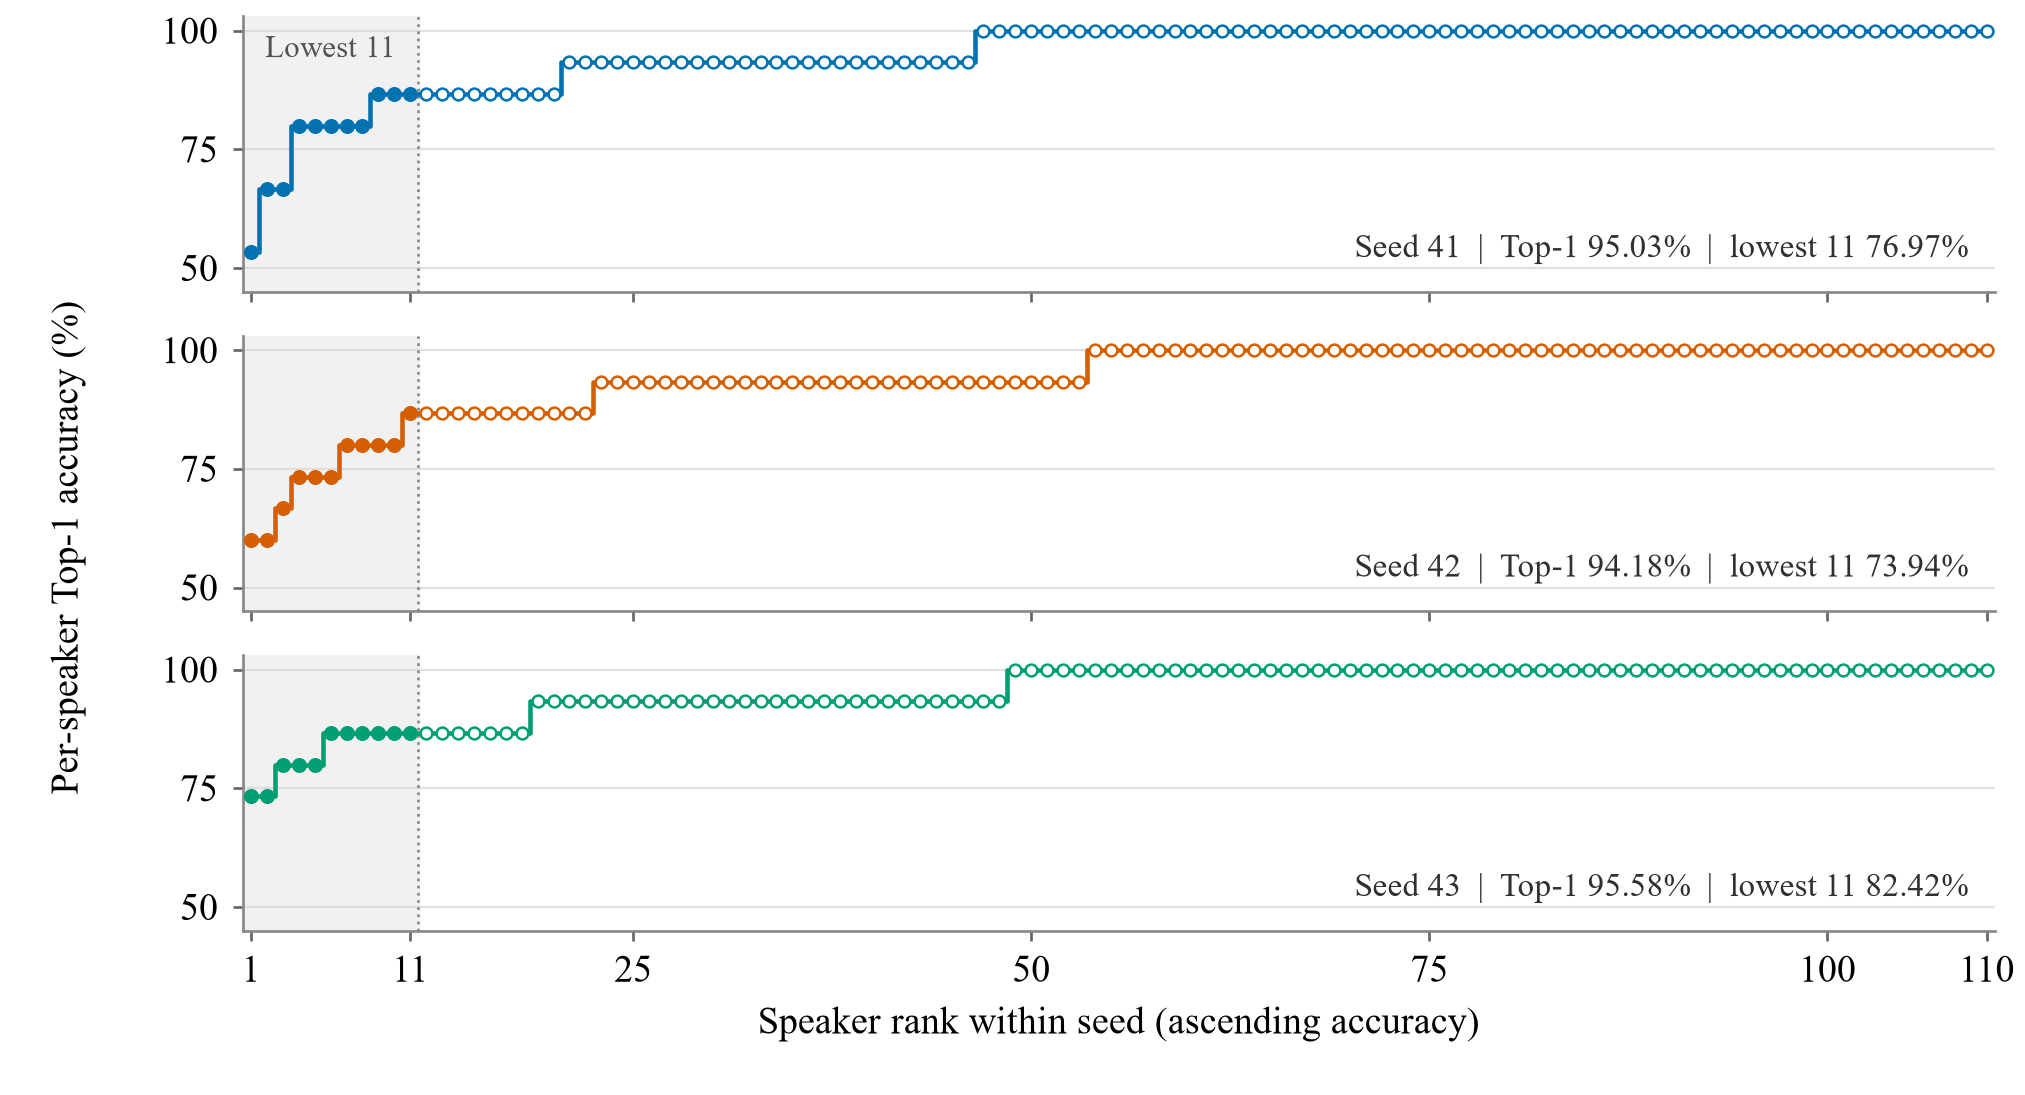
\includegraphics[width=\textwidth]{supplementary_methods_v3_assets/speaker_accuracy.png}
\caption{Per-speaker Top-1 accuracy for the formal 110-speaker test split and classifier training seeds 41--43. Speakers are independently ranked within each seed, with the lowest 11 ranks distinguished. Each speaker contributes 15 held-out utterance groups, so the plotted accuracies have discrete steps and should not be read as precise population-level speaker effects.}
\label{fig:sv4-speaker-accuracy}
\end{figure*}
% END V4-SPEAKER-FIGURE

\subsection{Across-seed summaries and hierarchical intervals}
For each metric $q$, Results reports the mean across seeds and, where shown, the sample standard deviation:
\begin{equation}
 \bar q=\frac{1}{3}\sum_{s=1}^{3}q_s,
 \qquad
 s_q=\sqrt{\frac{1}{2}\sum_{s=1}^{3}(q_s-\bar q)^2}.
 \label{eq:sv2-seeds}
\end{equation}
The seed-level predictions contain one record for each of the 1,650 test utterances. Training seeds label independently trained classifiers on the common split.

Within-seed Top-1 intervals used a two-level percentile bootstrap. A replicate first sampled 110 speakers with replacement. For each sampled speaker occurrence, it then sampled 15 test utterance groups with replacement from that speaker. The replicate accuracy was the mean correctness of the resulting 1,650 items. Repeated selections of a speaker received independent within-speaker draws.

The 2.5th and 97.5th percentiles defined each within-seed 95\% interval. Results uses the archived endpoints for each seed. The conservative lower endpoint was calculated as
\begin{equation}
 \ell_{\rm conservative}=\min(\ell_{41},\ell_{42},\ell_{43}),
 \label{eq:sv2-conservative}
\end{equation}
where $\ell_s$ is the lower endpoint for seed $s$. Across-seed sample variation and within-seed hierarchical resampling are therefore reported as distinct quantities. The minimum endpoint is a summary of the three within-seed bounds.

\section{Inference and receiver-side interface}
\label{sec:sv2-inference}

\subsection{Model loading and index decoding}
Inference loads the selected codec configuration, encoder weights, RVQ codebooks and decoder weights from a compatible checkpoint. Models are placed in evaluation mode and run without gradient tracking. The sender produces three-layer index sequences; the receiver restores the integer array, retrieves its codewords and decodes their sum.

The HuBERT teacher, adversarial discriminators and semantic-alignment projection are training components and are not required by the waveform inference path. The receiver-side classifier similarly uses only the trained feature encoders, fusion module, fusion head, label map and calibration metadata at prediction time.

The payload metadata specifies the number of indices and layer-by-frame dimensions used by unpacking. Compatible codebook ordering and checkpoint identity are required at the two endpoints: the same integer selects the same locally stored codeword at transmission and reception. Classification then receives those restored indices and the waveform reconstructed from them.

\subsection{Buffered waveform processing}
The implemented block interface accepts waveform lengths that are multiples of 320 samples. Its default block is 8,000 samples, or 0.5~s, corresponding nominally to 25 latent frames. A final short file-input block is zero-padded to the processing length.

The encoder contains bidirectional recurrence and noncausal convolutions. The interface accordingly encodes a buffered block once its waveform samples are available. This specifies the processing unit used by the software interface. The reconstruction measurements in Section~\ref{sec:sv2-evaluation} process complete utterances, and the resource profile in Section~\ref{sec:sv2-nas} times the stated encoder input.

At the receiver, restored indices are decoded into waveform blocks. Audio and token buffers retain the paired observations needed for classification. The token buffer keeps layer and time axes so that a classifier crop corresponds to the same interval as its audio crop.

\subsection{Classifier bundle and stream organization}
The exported seed-42 bundle contains the classifier state, the 110-class speaker-label map, preprocessing metadata and validation-fitted temperature. Preprocessing specifies 16-kHz audio, three RVQ layers, a nominal frame hop of 320 samples and a 48,000-sample classification window.

The implemented receiver maintains a separate audio buffer and token buffer for each incoming stream. Identity inference is performed on a stream's paired inputs before playback mixing. Stream identifiers select the corresponding buffers; the classifier's features are the received token sequence and its reconstructed waveform.

The default classification window is three seconds and is updated after each additional second of decoded audio. This window determines the speech context submitted to the classifier. The model returns margin-free fusion logits, calibrated probabilities from Equation~\ref{eq:sv2-probability}, the maximum-probability class and its mapped identity.

The interface can additionally display the largest probability and the gap between the two largest probabilities. These outputs summarize the probability distribution over the trained identity inventory. Label mapping, preprocessing and temperature are loaded with the checkpoint so that the displayed identity is tied to the same class ordering used in training.

% BEGIN V3-RECEIVER
\subsection{Worked receiver example and paired time windows}
Figure~\ref{fig:sv3-receiver} follows the data layouts at two scales. At the block scale, the nominal 0.5-s example contains $3\times25$ indices. Unpacking recovers these integers from 94 bytes, removes the two trailing padding bits and restores layer-major order. Codebook lookup and waveform decoding use this same recovered array, while the token path retains the integers for downstream feature extraction.

\begin{figure*}[t]
\centering
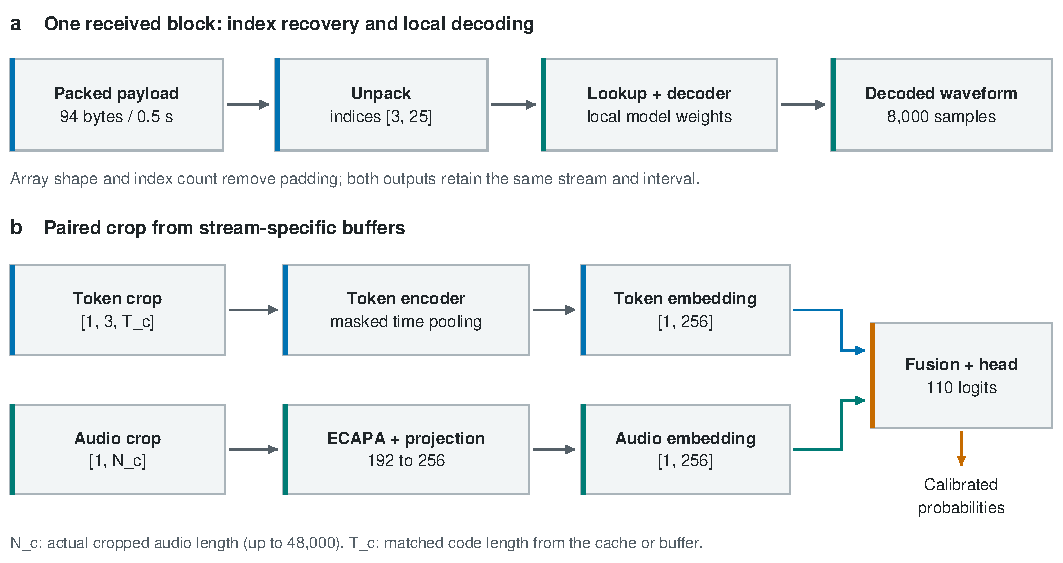
\includegraphics[width=\textwidth]{supplementary_methods_v3_assets/receiver_pairing.pdf}
\caption{Receiver data layouts and paired classification inputs. \textbf{a}, A nominal 0.5-s, three-layer block illustrates fixed-length packing, index recovery and local waveform reconstruction. \textbf{b}, A classification crop reads matching indices and reconstructed audio from one stream. $N_c$ and $T_c$ are the actual cropped sample and code lengths. Both branches produce 256-dimensional embeddings before gated fusion and the 110-class head. The diagram describes the processing interface and tensor dimensions, not an additional timing or multi-user experiment.}
\label{fig:sv3-receiver}
\end{figure*}

At the classification scale, the audio window contains up to 48,000 samples. The matching token crop is determined from the recorded audio and code lengths using Section~\ref{sec:sv2-speaker-protocol}; it is not obtained by unconditionally assigning 150 code frames to every three-second crop. This retains the correspondence when a cached utterance includes padding or a crop begins between nominal latent-frame boundaries. For a batch of one, the token tensor has shape $1\times3\times T_c$ and the waveform tensor has shape $1\times N_c$ before branch-specific preprocessing.

The stream identifier associates both buffers with the same incoming source, while sequence metadata identifies the received blocks. The identity decision is computed from the paired representation before playback mixing. Neither the stream identifier nor an independently transmitted identity embedding is supplied as a classifier feature. The label map converts the predicted class index to the corresponding trained speaker identity after calibrated fusion probabilities have been computed.
% END V3-RECEIVER

\section{Experimental correspondence and calculation conventions}
\label{sec:sv2-correspondence}

\subsection{Linking learning stages to measurements}
The experimental sequence supplies a direct correspondence between model states and reported quantities (Table~\ref{tab:sv2-crosswalk}). Architecture search selects the encoder configuration; joint codec training produces SCIT; channel-aware fine-tuning produces SCIT-LCA; and classifier training reads a cache generated by the frozen SCIT-LCA checkpoint. This ordering identifies the learned object evaluated at each stage.

\begin{table*}[t]
\centering
\caption{Correspondence between the main Results and the supplementary protocol. Every row refers to the retained experimental setting used by that result.}
\label{tab:sv2-crosswalk}
\small
\begin{tabularx}{\textwidth}{@{}p{0.22\textwidth}p{0.31\textwidth}Y@{}}
\toprule
Result & Experimental object & Supplementary specification\\
\midrule
Shared 1.5-kbit/s representation & Three 1024-entry codebooks at 50 latent frames/s & S1: residual quantization, rate calculation and bit packing\\
Encoder resource reductions & Reference encoder and selected configuration under common profiling conditions & S2: search schedule, ranking, parameter count, MACs and RTF\\
Matched-rate reconstruction & SCIT and pretrained external codecs on 300 test-clean utterances & S3 and S5: SCIT checkpoint, codec settings, metrics and utterance bootstrap\\
Channel-adaptation response & SCIT and SCIT-LCA on 2,620 paired test-clean utterances & S4--S5: adaptation objective, checkpoint, masks and signed differences\\
Receiver-side identification & Frozen SCIT-LCA cache and three trained 110-class classifiers & S6--S7: branches, split, optimization, calibration and uncertainty\\
Index reuse in the receiver & Matched received indices and decoded waveform & S1 and S8: payload recovery, classifier inputs and stream-specific buffering\\
\bottomrule
\end{tabularx}
\end{table*}

The external-codec comparison uses the base SCIT checkpoint, while the speaker study uses the channel-adapted checkpoint. Both share the selected architecture and three-layer index format. Their training histories and selected checkpoint steps are specified separately so that a model name identifies a reproducible experimental object.

\subsection{Aggregation, units and rounding}
All corpus-level reconstruction metrics use equal utterance weights. Speaker macro-F1 averages equally over classes; Top-1 and Top-5 average correctness over utterances; the lowest-decile score averages the 11 selected per-speaker accuracies. With 15 test items per identity, the speaker test population is class-balanced.

Results expresses accuracy, macro-F1, ECE and hierarchical interval endpoints as percentages where indicated. Multiplication by 100 is applied after aggregation. A difference between two percentage values is expressed in percentage points; resource reductions instead divide by the reference value as in Equation~\ref{eq:sv2-reduction}.

Unrounded archived values are retained for calculations, and displayed precision is applied at presentation. Reconstruction differences use the sign convention SCIT-LCA minus SCIT. Rounded point estimates can consequently yield a final displayed difference that differs by one unit in the last decimal place from subtracting already rounded table cells.

Nominal index rate, byte-aligned speech payload size, encoder RTF, waveform-block duration and classifier-window duration each have explicit definitions in the preceding sections. Reporting these quantities with their units associates each number with the measured operation or represented data.

\subsection{Experimental records and software environment}
The retained records include search configurations and profile tables; codec training and validation manifests; the selected architecture and checkpoint identifiers; utterance-level reconstruction measurements and channel seeds; the speaker split and cache manifests; per-seed classifier configurations and predictions; and calibration and label-map files.

The classifier environment records Python 3.10.19, PyTorch and torchaudio 2.9.1 with CUDA 12.8, and SpeechBrain 1.1.0. Encoder profiling additionally records THOP 0.1.1 and the RTX 5070 Ti. These versioned records identify the software used for the corresponding reported operations.

Together, the index definition, checkpoint sequence, matched evaluation populations and receiver input pairing connect the low-rate payload to its measured reconstruction and identification performance. The supplementary procedures provide the detailed experimental specification underlying the shared-representation results.

{\small
\begin{thebibliography}{00}
\bibitem{speechtokenizer}
X. Zhang, D. Zhang, S. Li, Y. Zhou, X. Qiu,
SpeechTokenizer: Unified Speech Tokenizer for Speech Large Language Models,
arXiv:2308.16692, 2023, revised 2024.
\url{https://arxiv.org/abs/2308.16692}.
\bibitem{hubert}
W.-N. Hsu, B. Bolte, Y.-H. H. Tsai, K. Lakhotia, R. Salakhutdinov, A. Mohamed,
HuBERT: Self-Supervised Speech Representation Learning by Masked Prediction of Hidden Units,
arXiv:2106.07447, 2021.
\url{https://arxiv.org/abs/2106.07447}.
\bibitem{ecapa}
B. Desplanques, J. Thienpondt, K. Demuynck,
ECAPA-TDNN: Emphasized Channel Attention, Propagation and Aggregation in TDNN Based Speaker Verification,
Proc. Interspeech 2020, pp. 3830--3834.
\url{https://doi.org/10.21437/Interspeech.2020-2650}.
\bibitem{librispeech}
V. Panayotov, G. Chen, D. Povey, S. Khudanpur,
LibriSpeech: An ASR corpus based on public domain audio books,
Proc. ICASSP, 2015. Corpus and reference:
\url{https://www.openslr.org/12}.
\bibitem{vctk}
J. Yamagishi, C. Veaux, K. MacDonald,
CSTR VCTK Corpus: English Multi-speaker Corpus for CSTR Voice Cloning Toolkit (version 0.92),
University of Edinburgh, 2019.
\url{https://doi.org/10.7488/ds/2645}.
\bibitem{dac}
R. Kumar, P. Seetharaman, A. Luebs, I. Kumar, K. Kumar,
High-Fidelity Audio Compression with Improved RVQGAN,
Advances in Neural Information Processing Systems 36, 2023.
\url{https://arxiv.org/abs/2306.06546}.
\bibitem{encodec}
A. D\'efossez, J. Copet, G. Synnaeve, Y. Adi,
High Fidelity Neural Audio Compression,
arXiv:2210.13438, 2022.
\url{https://arxiv.org/abs/2210.13438}.
\bibitem{stoi}
C. H. Taal, R. C. Hendriks, R. Heusdens, J. Jensen,
An Algorithm for Intelligibility Prediction of Time-Frequency Weighted Noisy Speech,
IEEE Transactions on Audio, Speech, and Language Processing 19 (7), 2011, pp. 2125--2136.
\url{https://doi.org/10.1109/TASL.2011.2114881}.
\bibitem{pesq}
ITU-T, Wideband extension to Recommendation P.862 for the assessment of wideband telephone networks and speech codecs,
Recommendation P.862.2, 2007.
\url{https://www.itu.int/rec/T-REC-P.862.2}.
\bibitem{arcface}
J. Deng, J. Guo, N. Xue, S. Zafeiriou,
ArcFace: Additive Angular Margin Loss for Deep Face Recognition,
Proc. IEEE/CVF Conference on Computer Vision and Pattern Recognition, 2019, pp. 4690--4699.
\url{https://doi.org/10.1109/CVPR.2019.00482}.
\end{thebibliography}

}
\end{document}
